% !TEX encoding = UTF-8 Unicode
% !TEX program = pdflatex
\documentclass[aspectratio=169, 10pt]{beamer}

% ==============================================================================
% 1. CẤU HÌNH GÓI VÀ BẢNG MÃ TIẾNG VIỆT
% ==============================================================================
\usepackage{cmap}
\usepackage[utf8]{inputenc}
\usepackage[T5]{fontenc}
\usepackage[utf8]{vietnam}
\usepackage{lmodern}
\usepackage{amsmath,amssymb}
\usepackage{tikz}
\usetikzlibrary{shapes.geometric, arrows.meta, positioning, calc, fit, chains, shadows}
\usepackage{booktabs}
\usepackage{tabularx}
\usepackage{tcolorbox}
\tcbuselibrary{skins}

% ==============================================================================
% 2. BẢNG MÀU VÀ GIAO DIỆN CHUẨN SLIDE 16:9
% ==============================================================================
\definecolor{PartyRed}{RGB}{185, 28, 28}       % Đỏ cờ Đảng (#B91C1C)
\definecolor{DarkRed}{RGB}{153, 27, 27}        % Đỏ sẫm tiêu đề (#991B1B)
\definecolor{GoldYellow}{RGB}{217, 119, 6}     % Vàng kim (#D97706)
\definecolor{NavyBlue}{RGB}{15, 23, 42}        % Xanh than tối (#0F172A)
\definecolor{CardBg}{RGB}{248, 250, 252}       % Nền thẻ sáng (#F8FAFC)
\definecolor{BorderGray}{RGB}{226, 232, 240}   % Viền thẻ (#E2E8F0)
\definecolor{TextDark}{RGB}{30, 41, 59}        % Chữ chính (#1E293B)
\definecolor{SuccessGreen}{RGB}{22, 101, 52}   % Xanh lá (#166534)
\definecolor{SkyBlue}{RGB}{2, 132, 199}        % Xanh dương (#0284C7)
\definecolor{IndigoColor}{RGB}{79, 70, 229}    % Chàm tím (#4F46E5)

\setbeamercolor{background canvas}{bg=white}
\setbeamercolor{normal text}{fg=TextDark}
\setbeamercolor{frametitle}{fg=DarkRed, bg=white}
\setbeamercolor{title}{fg=DarkRed, bg=white}
\setbeamercolor{subtitle}{fg=TextDark, bg=white}
\setbeamercolor{author}{fg=TextDark, bg=white}
\setbeamercolor{institute}{fg=TextDark, bg=white}
\setbeamercolor{date}{fg=TextDark, bg=white}

% Tắt thanh điều hướng mặc định của Beamer
\setbeamertemplate{navigation symbols}{}

% Tùy biến tiêu đề từng Slide (Frametitle) - Bỏ tiền tố Slide 1, 2...
\setbeamertemplate{frametitle}{
  \vspace{0.18cm}
  \begin{beamercolorbox}[wd=\paperwidth,leftskip=0.7cm,rightskip=0.7cm]{frametitle}
    {\fontsize{10.5pt}{12.5pt}\bfseries\color{DarkRed}\insertframetitle}
    \vskip 2pt
    \tikz \draw[PartyRed, line width=1.5pt] (0,0) -- (\paperwidth-1.4cm, 0);
  \end{beamercolorbox}
  \vspace{-0.32cm}
}

% Tùy biến Footer
\setbeamertemplate{footline}{
  \begin{beamercolorbox}[wd=\paperwidth,ht=0.38cm,dp=0.18cm,leftskip=0.7cm,rightskip=0.7cm]{footline}
    \fontsize{6.8pt}{8pt}\selectfont\color{gray}
    \textbf{Đề tài:} Hệ thống Quản lý Quần chúng Ưu tú (QLUT-Đảng)
    \hfill
    \textbf{Trường ĐH Tây Bắc} | Nhóm 02 \quad $\bullet$ \quad Trang \insertframenumber / \inserttotalframenumber
  \end{beamercolorbox}
}

% Tùy biến danh sách gạch đầu dòng
\setbeamertemplate{itemize item}{\color{PartyRed}$\blacktriangleright$}
\setbeamertemplate{itemize subitem}{\color{GoldYellow}$\bullet$}
\setbeamertemplate{enumerate item}{\color{PartyRed}\bfseries\insertenumlabel.}

% Hộp Card thông tin
\newtcolorbox{infoCard}[1][]{
  enhanced,
  colback=CardBg,
  colframe=BorderGray,
  boxrule=0.7pt,
  arc=3pt,
  left=4pt,right=4pt,top=3pt,bottom=3pt,
  fonttitle=\bfseries\color{DarkRed}\fontsize{8pt}{10pt}\selectfont,
  #1
}

\newtcolorbox{highlightCard}[2][]{
  enhanced,
  colback=PartyRed!4,
  colframe=PartyRed!80,
  title=#2,
  boxrule=0.8pt,
  arc=3pt,
  left=4pt,right=4pt,top=2.5pt,bottom=2.5pt,
  fonttitle=\bfseries\color{white}\fontsize{7.8pt}{9.8pt}\selectfont,
  colbacktitle=PartyRed,
  #1
}

\newtcolorbox{greenCard}[2][]{
  enhanced,
  colback=SuccessGreen!4,
  colframe=SuccessGreen!80,
  title=#2,
  boxrule=0.8pt,
  arc=3pt,
  left=4pt,right=4pt,top=2.5pt,bottom=2.5pt,
  fonttitle=\bfseries\color{white}\fontsize{7.8pt}{9.8pt}\selectfont,
  colbacktitle=SuccessGreen,
  #1
}

% ==============================================================================
% THÔNG TIN BÁO CÁO
% ==============================================================================
\title{HỆ THỐNG QUẢN LÝ QUẦN CHÚNG ƯU TÚ}
\subtitle{BÁO CÁO BÀI TẬP LỚN MÔN HỌC (QLUT-ĐẢNG)}
\author{Nhóm 02}
\institute{Khoa Công nghệ Thông tin --- Trường Đại học Tây Bắc}
\date{Tháng 08/2026}

% ==============================================================================
% NỘI DUNG CHÍNH CỦA SLIDE
% ==============================================================================
\begin{document}

% ------------------------------------------------------------------------------
% SLIDE BÌA (TITLE SLIDE)
% ------------------------------------------------------------------------------
\begin{frame}[plain]
  \vspace{0.2cm}
  \centering
  {\fontsize{9pt}{11pt}\selectfont\bfseries\color{DarkRed} BỘ GIÁO DỤC VÀ ĐÀO TẠO --- TRƯỜNG ĐẠI HỌC TÂY BẮC}\\
  {\fontsize{8pt}{10pt}\selectfont\bfseries\color{TextDark} KHOA CÔNG NGHỆ THÔNG TIN}

  \vspace{0.15cm}
  \tikz \draw[PartyRed, line width=1.5pt] (0,0) -- (12.5cm, 0);
  \vspace{0.15cm}

  {\fontsize{14pt}{18pt}\selectfont\bfseries\color{DarkRed} HỆ THỐNG QUẢN LÝ QUẦN CHÚNG ƯU TÚ}

  \vspace{0.08cm}
  {\fontsize{9pt}{11pt}\selectfont\bfseries\color{GoldYellow} BÁO CÁO BÀI TẬP LỚN MÔN HỌC (QLUT-ĐẢNG)}

  \vspace{0.2cm}
  \begin{columns}[T]
    \begin{column}{0.48\textwidth}
      \centering
      \begin{infoCard}
        \fontsize{7.2pt}{9pt}\selectfont
        \textbf{Giảng viên hướng dẫn:}\\
        ThS. Đặng Thị Vân Chi\\
        \textit{Khoa Công nghệ Thông tin}
      \end{infoCard}
    \end{column}
    \begin{column}{0.48\textwidth}
      \begin{infoCard}
        \fontsize{7.2pt}{9pt}\selectfont
        \textbf{Sinh viên thực hiện (Nhóm 02):}\\
        1. Lò Mạnh Đạt (2023A0861) - Trưởng nhóm\\
        2. Nguyễn Huy Hoàng (2023A0875)\\
        3. Tòng Lưu Anh Tú (2023A0937)\\
        4. Phạm Thị Thanh Hảo (2023A0869)
      \end{infoCard}
    \end{column}
  \end{columns}

  \vspace{0.15cm}
  {\fontsize{7pt}{8.5pt}\selectfont\color{gray} Sơn La, Tháng 08/2026}
\end{frame}

% ------------------------------------------------------------------------------
% 1. 6 ĐIỂM NGHẼN THỰC TẾ VÀ MỤC TIÊU SỐ HÓA HỆ THỐNG
% ------------------------------------------------------------------------------
\begin{frame}{6 ĐIỂM NGHẼN THỰC TẾ VÀ MỤC TIÊU SỐ HÓA HỆ THỐNG}
  \begin{columns}[T]
    \begin{column}{0.48\textwidth}
      \begin{highlightCard}{6 Điểm nghẽn Quản lý Thủ công}
        \fontsize{6.8pt}{8.5pt}\selectfont
        \begin{itemize}
          \setlength{\itemsep}{1.2pt}
          \item \textbf{Thất lạc \& Hư hỏng}: Hồ sơ giấy nhiều năm dễ ẩm mốc, rách hỏng khi luân chuyển giữa các cấp.
          \item \textbf{Chậm trễ đối soát}: Mất 45--60 phút/bộ hồ sơ, dễ bỏ sót lỗi thiếu chữ ký, con dấu.
          \item \textbf{Thiếu minh bạch}: Quần chúng không nắm được hồ sơ đang ở bước nào trong quy trình.
          \item \textbf{Phân tán dữ liệu}: File Excel rời rạc gây trùng lặp, sai lệch thông tin cá nhân.
          \item \textbf{Lỗi nhập liệu Excel}: Tệp nộp lên bị lệch cột, viết tắt hoặc khuyết tiêu đề.
          \item \textbf{Lãng phí in ấn}: Sai một lỗi nhỏ phải in lại toàn bộ biểu mẫu nhiều trang.
        \end{itemize}
      \end{highlightCard}
    \end{column}
    \begin{column}{0.48\textwidth}
      \begin{greenCard}{Mục tiêu Đột phá của Hệ thống QLUT-Đảng}
        \fontsize{6.8pt}{8.5pt}\selectfont
        \begin{itemize}
          \setlength{\itemsep}{1.5pt}
          \item \textbf{Số hóa 100\% quy trình}: Quản lý trọn vòng đời từ nộp đơn $\to$ rèn luyện $\to$ kết nạp.
          \item \textbf{Ứng dụng Edge AI tại Client}: Xử lý trực tiếp trên trình duyệt, không tốn chi phí thuê máy chủ GPU đắt đỏ.
          \item \textbf{Hiệu năng thiết kế vượt trội}:
                \begin{center}
                  \tikz[scale=0.85, every node/.style={transform shape, font=\tiny\bfseries}]{
                    \node[draw=SuccessGreen, fill=green!10, rounded corners=2pt, minimum width=1.5cm, align=center] (k1) {Tải Web\\$<0.3$s};
                    \node[draw=PartyRed, fill=red!10, rounded corners=2pt, minimum width=1.5cm, align=center, right=0.2cm of k1] (k2) {AI OCR\\$<2.5$s};
                    \node[draw=GoldYellow, fill=yellow!10, rounded corners=2pt, minimum width=1.5cm, align=center, right=0.2cm of k2] (k3) {Xuất PDF\\$<1.0$s};
                  }
                \end{center}
          \item \textbf{Cơ sở dữ liệu 3NF}: Chuẩn hóa dữ liệu tập trung, phân quyền RBAC 3 vai trò.
        \end{itemize}
      \end{greenCard}
    \end{column}
  \end{columns}
\end{frame}

% ------------------------------------------------------------------------------
% 2. QUY TRÌNH NGHIỆP VỤ 5 BƯỚC VÀ PHÂN QUYỀN RBAC 3 VAI TRÒ
% ------------------------------------------------------------------------------
\begin{frame}{QUY TRÌNH NGHIỆP VỤ 5 BƯỚC VÀ PHÂN QUYỀN RBAC 3 VAI TRÒ}
  % Sơ đồ 5 bước liên hoàn
  \begin{center}
    \tikz[scale=0.88, every node/.style={transform shape, font=\fontsize{6pt}{7.5pt}\selectfont\bfseries, align=center, minimum height=0.6cm, rounded corners=2pt}]{
      \node[draw=PartyRed, fill=red!10, minimum width=2.4cm] (s1) {Bước 1\\Nộp đơn online};
      \node[draw=GoldYellow, fill=yellow!10, minimum width=2.4cm, right=0.2cm of s1] (s2) {Bước 2\\Duyệt cảm tình};
      \node[draw=SkyBlue, fill=blue!10, minimum width=2.4cm, right=0.2cm of s2] (s3) {Bước 3\\Theo dõi rèn luyện};
      \node[draw=IndigoColor, fill=IndigoColor!10, minimum width=2.4cm, right=0.2cm of s3] (s4) {Bước 4\\Thẩm định minh chứng};
      \node[draw=SuccessGreen, fill=green!10, minimum width=2.4cm, right=0.2cm of s4] (s5) {Bước 5\\Quyết định kết nạp};
      \draw[-Latex, thick, PartyRed] (s1) -- (s2);
      \draw[-Latex, thick, GoldYellow] (s2) -- (s3);
      \draw[-Latex, thick, SkyBlue] (s3) -- (s4);
      \draw[-Latex, thick, IndigoColor] (s4) -- (s5);
    }
  \end{center}
  \vspace{-0.2cm}
  \begin{columns}[T]
    \begin{column}{0.50\textwidth}
      \begin{infoCard}
        \textbf{\color{DarkRed}Quy trình 5 Bước Chuẩn hóa (HD 01-HD/TW)}
        \vspace{1pt}
        \fontsize{6.8pt}{8.5pt}\selectfont
        \begin{enumerate}
          \setlength{\itemsep}{1pt}
          \item \textbf{Nộp đơn}: Điền form trực tuyến (OCR CCCD tự điền).
          \item \textbf{Cảm tình Đảng}: Bí thư thẩm định \& duyệt danh sách.
          \item \textbf{Rèn luyện}: Ghi nhận học lớp Đảng \& xếp loại đoàn viên.
          \item \textbf{Thẩm định}: AI quét bắt lỗi thiếu thông tin minh chứng.
          \item \textbf{Kết nạp}: Đảng ủy duyệt, xuất 8 biểu mẫu PDF.
        \end{enumerate}
      \end{infoCard}
    \end{column}
    \begin{column}{0.48\textwidth}
      \begin{highlightCard}{Phân quyền RBAC 3 Vai trò Người dùng}
        \fontsize{6.8pt}{8.5pt}\selectfont
        \begin{itemize}
          \setlength{\itemsep}{1.5pt}
          \item \textbf{1. Sinh viên / Quần chúng}: Nộp đơn, xem Timeline 5 bước thời gian thực, gửi đề xuất sửa đổi thông tin.
          \item \textbf{2. Quản lý (Bí thư / Cán bộ)}: Duyệt đơn 2 Tab Cũ--Mới, sửa nhanh Autosave, xuất báo cáo \& 8 PDF.
          \item \textbf{3. Quản trị viên (Admin)}: Cấp quyền, đặt lại mật khẩu, cấu hình hệ thống, an ninh bảo mật.
        \end{itemize}
        \textit{\color{gray} Nguyên tắc: AI chỉ khuyến nghị; quyền phê duyệt thuộc cán bộ.}
      \end{highlightCard}
    \end{column}
  \end{columns}
\end{frame}

% ------------------------------------------------------------------------------
% 3. KIẾN TRÚC HỆ THỐNG PHÂN TẦNG LAI VÀ 3 TRỤ CỘT CÔNG NGHỆ
% ------------------------------------------------------------------------------
\begin{frame}{KIẾN TRÚC HỆ THỐNG PHÂN TẦNG LAI VÀ 3 TRỤ CỘT CÔNG NGHỆ}
  % Sơ đồ 3 trụ cột kỹ thuật
  \begin{center}
    \tikz[scale=0.88, every node/.style={transform shape, font=\fontsize{6pt}{7.5pt}\selectfont\bfseries, align=center, minimum height=0.55cm, rounded corners=2pt}]{
      \node[draw=PartyRed, fill=red!10, minimum width=3.4cm] (c1) {TRỤ CỘT 1: EDGE AI\\WASM OCR + Camera + Canvas};
      \node[draw=GoldYellow, fill=yellow!10, minimum width=3.4cm, right=0.25cm of c1] (c2) {TRỤ CỘT 2: MULTI-AGENT\\4 Agent Thẩm định + Map Excel};
      \node[draw=SuccessGreen, fill=green!10, minimum width=3.4cm, right=0.25cm of c2] (c3) {TRỤ CỘT 3: PYTHON SERVICE\\ReportLab PDF + openpyxl};
    }
  \end{center}
  \vspace{-0.2cm}
  \begin{columns}[T]
    \begin{column}{0.48\textwidth}
      \begin{infoCard}
        \textbf{\color{DarkRed}Phân định Nhiệm vụ Kỹ thuật}
        \fontsize{6.8pt}{8.5pt}\selectfont
        \begin{itemize}
          \setlength{\itemsep}{1.5pt}
          \item \textbf{Trụ cột 1 (Edge AI)}: Xử lý tại Client RAM, đo nét Camera, bóc tách CCCD tự điền form, cắt ảnh 3x4.
          \item \textbf{Trụ cột 2 (Multi-Agent)}: Bộ tác tử thông minh soi lỗi trường khuyết và tự khớp cột Excel.
          \item \textbf{Trụ cột 3 (Python Service)}: Server Flask :5000 chuyên xuất 8 mẫu phiếu PDF và Excel 35 cột.
        \end{itemize}
      \end{infoCard}
    \end{column}
    \begin{column}{0.48\textwidth}
      \begin{greenCard}{Tầng Điều phối PHP Core \& MySQL 3NF}
        \fontsize{6.8pt}{8.5pt}\selectfont
        \begin{itemize}
          \setlength{\itemsep}{1.5pt}
          \item \textbf{PHP Backend}: Quản lý Controller, phân quyền RBAC, định tuyến dữ liệu qua Proxy Bridge (\texttt{api\_proxy.php}).
          \item \textbf{MySQL 3NF}: Lưu trữ tập trung 9 bảng dữ liệu, đảm bảo toàn vẹn tham chiếu.
          \item \textbf{Hiệu quả}: Tách biệt tải nặng khỏi máy chủ Web, hệ thống luôn phản hồi dưới 0.3 giây.
        \end{itemize}
      \end{greenCard}
    \end{column}
  \end{columns}
\end{frame}

% ------------------------------------------------------------------------------
% 4. CHI TIẾT KIẾN TRÚC PHÂN TẦNG LAI VÀ LUỒNG ĐIỀU PHỐI DỮ LIỆU (SAU SLIDE 3)
% ------------------------------------------------------------------------------
\begin{frame}{CHI TIẾT KIẾN TRÚC PHÂN TẦNG LAI VÀ LUỒNG ĐIỀU PHỐI DỮ LIỆU}
  % Sơ đồ Luồng phân tầng và phân lập tải
  \begin{center}
    \tikz[scale=0.88, every node/.style={transform shape, font=\fontsize{5.8pt}{7.2pt}\selectfont\bfseries, align=center, minimum height=0.55cm, rounded corners=2pt}]{
      \node[draw=NavyBlue, fill=blue!10, minimum width=2.6cm] (n1) {1. Client Browser\\(Edge AI \& WebAssembly)};
      \node[draw=DarkRed, fill=red!10, minimum width=2.6cm, right=0.35cm of n1] (n2) {2. PHP Core Backend\\(Controller \& RBAC)};
      \node[draw=GoldYellow, fill=yellow!10, minimum width=2.6cm, right=0.35cm of n2] (n4) {3. MySQL CSDL\\(9 Bảng Dữ liệu 3NF)};
      \node[draw=SuccessGreen, fill=green!10, minimum width=2.6cm, right=0.35cm of n4] (n3) {4. Python Microservice\\(Flask :5000 Engine)};
      \draw[-Latex, thick, NavyBlue] (n1) -- (n2);
      \draw[-Latex, thick, GoldYellow] (n2) -- (n4);
      \draw[-Latex, thick, DarkRed] (n4) -- (n3);
      \path (n1.north east) -- node[above=1.5pt, font=\fontsize{4.5pt}{5.5pt}\selectfont, color=NavyBlue]{AJAX JSON} (n2.north west);
      \path (n2.north east) -- node[above=1.5pt, font=\fontsize{4.5pt}{5.5pt}\selectfont, color=GoldYellow!80!black]{PDO Query} (n4.north west);
      \path (n4.north east) -- node[above=1.5pt, font=\fontsize{4.5pt}{5.5pt}\selectfont, color=DarkRed]{REST Proxy} (n3.north west);
      \draw[-Latex, thick, SuccessGreen, dashed] (n3.south) to[bend left=20] node[below=1.5pt, font=\fontsize{4.5pt}{5.5pt}\selectfont, color=SuccessGreen]{Binary Stream PDF/Excel} (n1.south);
    }
  \end{center}
  \vspace{-0.2cm}
  \begin{columns}[T]
    \begin{column}{0.48\textwidth}
      \begin{highlightCard}{Cơ chế Phân lập Trọng tải (Workload Decoupling)}
        \fontsize{6.8pt}{8.5pt}\selectfont
        \begin{itemize}
          \setlength{\itemsep}{1.2pt}
          \item \textbf{Tách biệt tải tính toán}: Tách rời tác vụ tương tác I/O (PHP) và tác vụ tính toán nặng CPU (Client AI \& Python Service).
          \item \textbf{Giải phóng máy chủ Web}: Web Server PHP không bao giờ bị nghẽn CPU khi hàng trăm sinh viên quét ảnh CCCD hay xuất báo cáo.
          \item \textbf{Phản hồi $<0.3$s}: Đảm bảo trải nghiệm người dùng luôn mượt mà.
        \end{itemize}
      \end{highlightCard}
    \end{column}
    \begin{column}{0.48\textwidth}
      \begin{greenCard}{Vòng đời Điều phối Sự kiện (Event Lifecycle)}
        \fontsize{6.8pt}{8.5pt}\selectfont
        \begin{itemize}
          \setlength{\itemsep}{1.2pt}
          \item \textbf{1. Tiền xử lý}: Client AI bóc tách CCCD trong RAM $\to$ Gửi dữ liệu sạch JSON lên máy chủ PHP.
          \item \textbf{2. Kiểm soát \& Lưu trữ}: PHP xác thực Token, phân quyền RBAC và ghi nhận vào MySQL 3NF an toàn.
          \item \textbf{3. Xuất tệp tức thì}: PHP kích hoạt Proxy Bridge $\to$ Python Flask render file nhị phân $\to$ Trả về Client tải xuống ngay.
        \end{itemize}
      \end{greenCard}
    \end{column}
  \end{columns}
\end{frame}

% ------------------------------------------------------------------------------
% 5. THIẾT KẾ CƠ SỞ DỮ LIỆU CHUẨN HÓA 3NF VÀ LƯỢC ĐỒ 9 BẢNG
% ------------------------------------------------------------------------------
\begin{frame}{THIẾT KẾ CƠ SỞ DỮ LIỆU CHUẨN HÓA 3NF VÀ LƯỢC ĐỒ 9 BẢNG}
  \begin{columns}[T]
    \begin{column}{0.52\textwidth}
      \begin{highlightCard}{Bảng Trung tâm \texttt{doi\_tuong} (35 Trường)}
        \fontsize{6.8pt}{8.2pt}\selectfont
        Quản lý trọn vẹn thông tin đối tượng qua 5 giai đoạn:
        \begin{itemize}
          \setlength{\itemsep}{1pt}
          \item \textbf{Định danh cá nhân}: Họ tên, Mã SV, CCCD, Ngày sinh, Giới tính, Quê quán, Lớp học, Dân tộc, Tôn giáo, SĐT, Email.
          \item \textbf{Tổ chức Đảng}: Chi bộ quản lý, Đảng viên kèm cặp.
          \item \textbf{Mốc thời gian}: Ngày nộp đơn, Ngày cảm tình, Ngày học lớp nhận thức Đảng (Lớp 1 \& 2).
          \item \textbf{Đánh giá \& Minh chứng}: Điểm rèn luyện, Xếp loại đoàn viên, Đường dẫn tệp minh chứng.
          \item \textbf{Trạng thái vòng đời}: Chờ duyệt $\to$ Theo dõi $\to$ Kết nạp.
        \end{itemize}
      \end{highlightCard}
    \end{column}
    \begin{column}{0.46\textwidth}
      \begin{infoCard}
        \textbf{\color{DarkRed}Lược đồ ERD 8 Bảng Vệ tinh}
        \begin{center}
          \tikz[scale=0.68, every node/.style={transform shape, font=\tiny\bfseries, align=center}]{
            % Bảng trung tâm
            \node[draw=PartyRed, fill=red!15, line width=0.8pt, rounded corners=2pt, minimum width=2.2cm, minimum height=1.5cm] (main) {\texttt{doi\_tuong}\\(Trung tâm\\35 cột)};

            % 4 Bảng bên trái
            \node[draw=NavyBlue, fill=blue!5, rounded corners=2pt, minimum width=1.45cm, left=0.45cm of main.north west, anchor=east] (t1) {\texttt{nguoi\_dung}};
            \node[draw=NavyBlue, fill=blue!5, rounded corners=2pt, minimum width=1.45cm, below=0.12cm of t1] (t2) {\texttt{chi\_bo}};
            \node[draw=NavyBlue, fill=blue!5, rounded corners=2pt, minimum width=1.45cm, below=0.12cm of t2] (t3) {\texttt{yeu\_cau\_cap\_nhat}};
            \node[draw=NavyBlue, fill=blue!5, rounded corners=2pt, minimum width=1.45cm, below=0.12cm of t3] (t4) {\texttt{lich\_su}};

            % 4 Bảng bên phải
            \node[draw=NavyBlue, fill=blue!5, rounded corners=2pt, minimum width=1.45cm, right=0.45cm of main.north east, anchor=west] (t5) {\texttt{dang\_ky\_doi\_tuong}};
            \node[draw=NavyBlue, fill=blue!5, rounded corners=2pt, minimum width=1.45cm, below=0.12cm of t5] (t6) {\texttt{dang\_vien}};
            \node[draw=NavyBlue, fill=blue!5, rounded corners=2pt, minimum width=1.45cm, below=0.12cm of t6] (t7) {\texttt{edge\_ai\_logs}};
            \node[draw=NavyBlue, fill=blue!5, rounded corners=2pt, minimum width=1.45cm, below=0.12cm of t7] (t8) {\texttt{cai\_dat}};

            % Mũi tên kết nối 8 bảng
            \draw[-Latex, thick, gray] (t1.east) -- (main.160);
            \draw[-Latex, thick, gray] (t2.east) -- (main.180);
            \draw[-Latex, thick, gray] (t3.east) -- (main.200);
            \draw[-Latex, thick, gray] (t4.east) -- (main.220);

            \draw[-Latex, thick, gray] (t5.west) -- (main.20);
            \draw[-Latex, thick, gray] (t6.west) -- (main.0);
            \draw[-Latex, thick, gray] (t7.west) -- (main.340);
            \draw[-Latex, thick, gray] (t8.west) -- (main.320);
          }
        \end{center}
        \fontsize{6.3pt}{7.6pt}\selectfont
        \textit{Khóa ngoại (\texttt{ON DELETE RESTRICT/CASCADE}) ràng buộc toàn vẹn 8 bảng vệ tinh với bảng trung tâm.}
      \end{infoCard}
    \end{column}
  \end{columns}
\end{frame}

% ------------------------------------------------------------------------------
% 6. CƠ CHẾ BẢO MẬT ĐA TẦNG VÀ AN TOÀN DỮ LIỆU CÁ NHÂN
% ------------------------------------------------------------------------------
\begin{frame}{CƠ CHẾ BẢO MẬT ĐA TẦNG VÀ AN TOÀN DỮ LIỆU CÁ NHÂN}
  % Sơ đồ 4 lớp khiên bảo mật
  \begin{center}
    \tikz[scale=0.88, every node/.style={transform shape, font=\fontsize{6pt}{7.5pt}\selectfont\bfseries, align=center, minimum height=0.55cm, rounded corners=2pt}]{
      \node[draw=PartyRed, fill=red!10, minimum width=2.4cm] (k1) {Khiên 1: Băm mật khẩu\\BCRYPT (Cost=10)};
      \node[draw=GoldYellow, fill=yellow!10, minimum width=2.4cm, right=0.2cm of k1] (k2) {Khiên 2: Chống SQLi\\PDO Prepared Stmts};
      \node[draw=SkyBlue, fill=blue!10, minimum width=2.4cm, right=0.2cm of k2] (k3) {Khiên 3: XSS / CSRF\\Filter Output \& Tokens};
      \node[draw=SuccessGreen, fill=green!10, minimum width=2.4cm, right=0.2cm of k3] (k4) {Khiên 4: RAM Client\\Bảo vệ dữ liệu CCCD};
      \draw[-Latex, thick, gray] (k1) -- (k2);
      \draw[-Latex, thick, gray] (k2) -- (k3);
      \draw[-Latex, thick, gray] (k3) -- (k4);
    }
  \end{center}
  \vspace{-0.2cm}
  \begin{columns}[T]
    \begin{column}{0.48\textwidth}
      \begin{highlightCard}{Bảo vệ Dữ liệu \& Chống Tấn công}
        \fontsize{6.8pt}{8.5pt}\selectfont
        \begin{itemize}
          \setlength{\itemsep}{1.2pt}
          \item \textbf{BCRYPT ($Cost=10$)}: Băm 1 chiều, chống giải mã ngược.
          \item \textbf{PDO Prepared Statements}: Tham số hóa 100\% truy vấn, triệt tiêu nguy cơ SQL Injection.
          \item \textbf{Lọc XSS \& CSRF Token}: Tự động làm sạch dữ liệu đầu ra và cấp mã Token ngẫu nhiên cho form.
          \item \textbf{Chống Session Fixation}: Tự đổi Session ID khi login.
        \end{itemize}
      \end{highlightCard}
    \end{column}
    \begin{column}{0.48\textwidth}
      \begin{greenCard}{Kiểm soát Truy cập \& Quyền riêng tư}
        \fontsize{6.8pt}{8.5pt}\selectfont
        \begin{itemize}
          \setlength{\itemsep}{1.2pt}
          \item \textbf{Rate Limiting}: Tự động khóa tạm thời khi nhập sai mật khẩu quá 5 lần trong 15 phút.
          \item \textbf{Kiểm duyệt tệp tải lên}: Chỉ cho phép PDF, JPEG, PNG.
          \item \textbf{An toàn dữ liệu cá nhân (Edge AI)}:
                \begin{itemize}
                  \item Xử lý ảnh CCCD trực tiếp tại RAM máy người dùng.
                  \item Không lưu trữ ảnh CCCD thô trên máy chủ web.
                \end{itemize}
        \end{itemize}
      \end{greenCard}
    \end{column}
  \end{columns}
\end{frame}

% ------------------------------------------------------------------------------
% 7. CHI TIẾT CƠ CHẾ BẢO MẬT: BẢO VỆ PHIÊN, RATE LIMITING VÀ CÔ LẬP DỮ LIỆU
% ------------------------------------------------------------------------------
\begin{frame}{CHI TIẾT BẢO MẬT: BẢO VỆ PHIÊN, RATE LIMITING \& CÔ LẬP DỮ LIỆU}
  \begin{columns}[T]
    \begin{column}{0.48\textwidth}
      \begin{infoCard}
        \textbf{\color{DarkRed}Kiểm soát Phiên \& Chống Leo thang Quyền}
        \fontsize{6.8pt}{8.5pt}\selectfont
        \begin{itemize}
          \setlength{\itemsep}{1.5pt}
          \item \textbf{RBAC Middleware (\texttt{requireRole})}: Mọi request quản trị đều bị chặn bắt tại cổng, đối chiếu session \& quyền trước khi vào Controller.
          \item \textbf{Session Regeneration}: Tự hủy Session ID cũ, cấp ID ngẫu nhiên mới ngay khi đăng nhập $\to$ Triệt tiêu Session Hijacking.
          \item \textbf{Rate Limiting CSDL}: Ghi nhận IP \& mốc thời gian, tự khóa tài khoản 15 phút nếu nhập sai quá 5 lần.
        \end{itemize}
      \end{infoCard}
    \end{column}
    \begin{column}{0.48\textwidth}
      \begin{greenCard}{Cô lập Bộ nhớ \& Bảo vệ Dữ liệu Nhạy cảm}
        \fontsize{6.8pt}{8.5pt}\selectfont
        \begin{itemize}
          \setlength{\itemsep}{1.5pt}
          \item \textbf{Tham số hóa PDO BindParam}: Tách biệt tuyệt đối giữa lệnh SQL và dữ liệu nhập $\to$ Vô hiệu hóa mọi mã độc SQL Injection.
          \item \textbf{Cô lập RAM Client (WASM Sandboxing)}: Web Worker bóc tách CCCD trong luồng độc lập; tự dọn rác bộ nhớ (Garbage Collection) ngay khi xong việc.
          \item \textbf{Không lộ lọt dữ liệu}: Dữ liệu thẻ CCCD không bao giờ bị lưu vết ở server.
        \end{itemize}
      \end{greenCard}
    \end{column}
  \end{columns}
\end{frame}

% ------------------------------------------------------------------------------
% 8. GIAO DIỆN QUẢN TRỊ: DASHBOARD, DUYỆT 2 TAB VÀ SỬA NHANH (2 ẢNH)
% ------------------------------------------------------------------------------
\begin{frame}{GIAO DIỆN QUẢN TRỊ: DASHBOARD, DUYỆT 2 TAB VÀ SỬA NHANH}
  \begin{columns}[T]
    \begin{column}{0.49\textwidth}
      \begin{highlightCard}{Giao diện Người dùng (Sinh viên / Quần chúng)}
        \centering
        \vspace{1pt}
        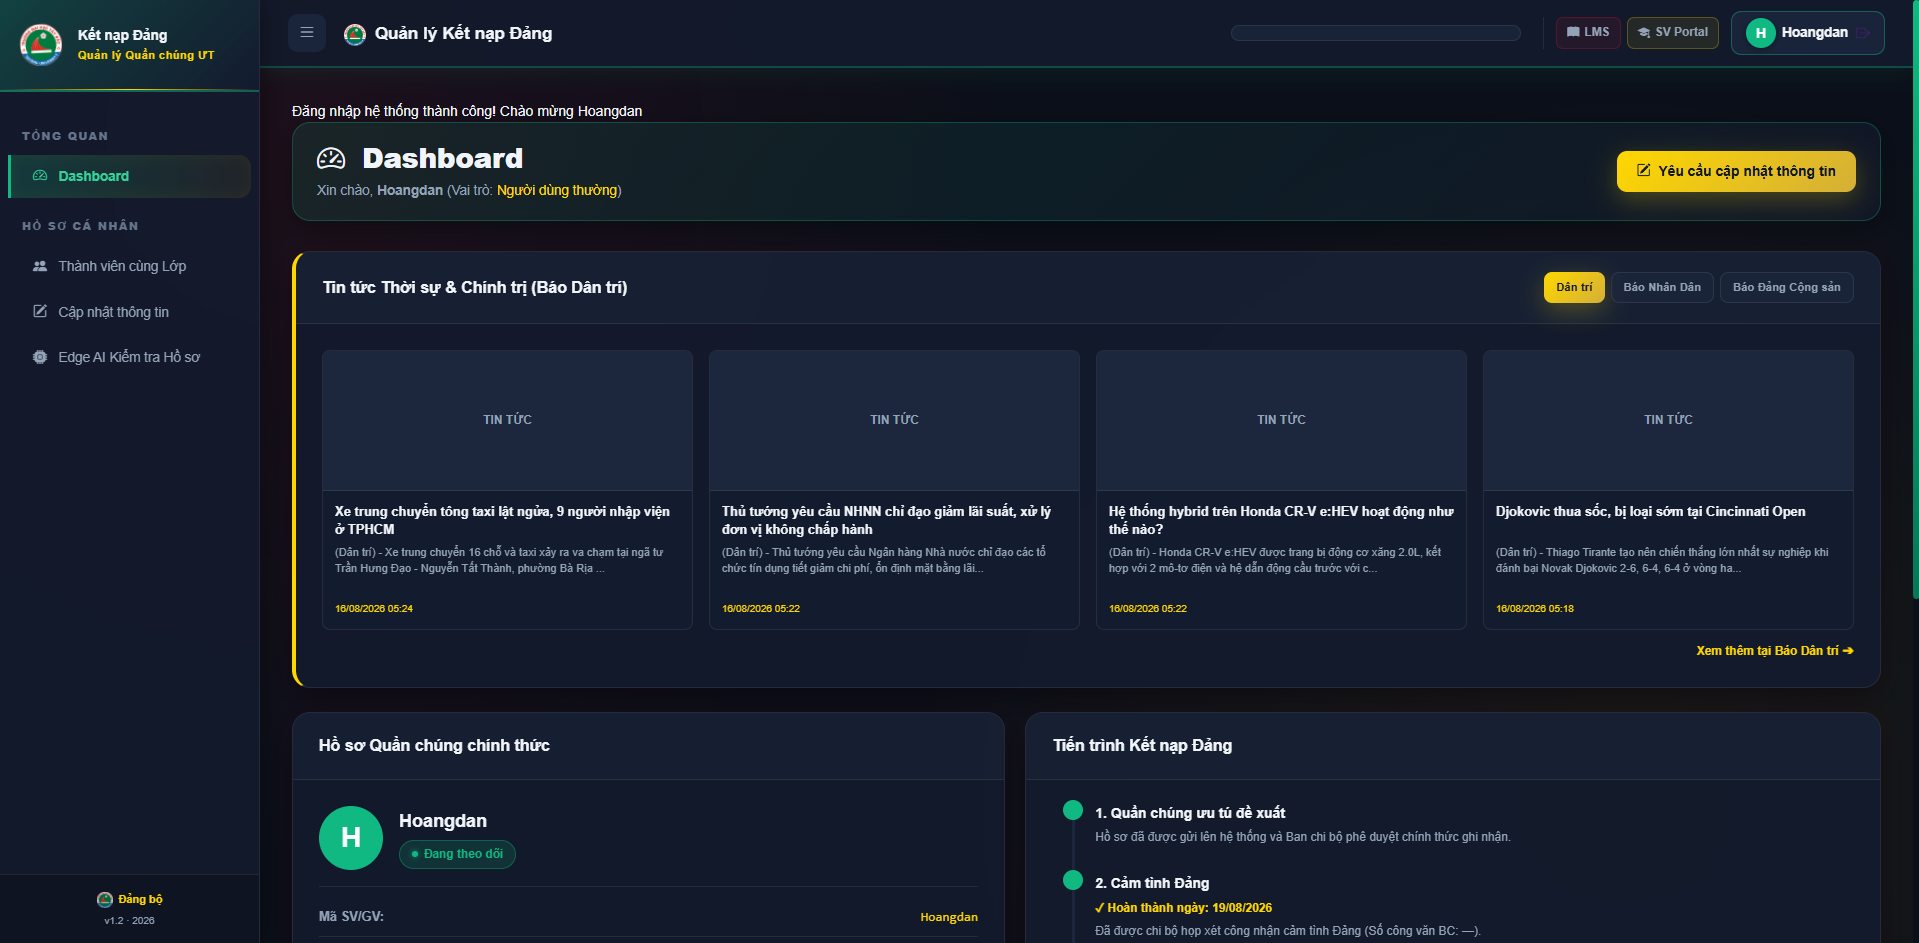
\includegraphics[width=0.98\linewidth, height=2.3cm, keepaspectratio]{giaodiennguoidung.png}
        \vspace{1pt}
        \fontsize{6.2pt}{7.8pt}\selectfont
        \begin{itemize}
          \setlength{\itemsep}{0.5pt}
          \item \textbf{Profile Card}: Ảnh thẻ 3x4, họ tên, chi bộ, trạng thái hồ sơ.
          \item \textbf{Timeline 5 bước}: Trực quan hóa tiến trình theo thời gian thực.
          \item \textbf{Danh sách cùng lớp}: Tra cứu bạn bè đã được duyệt.
          \item \textbf{Gửi đề xuất sửa đổi}: Chủ động xin cập nhật SĐT, Email, Lớp.
        \end{itemize}
      \end{highlightCard}
    \end{column}
    \begin{column}{0.49\textwidth}
      \begin{greenCard}{Giao diện Quản lý (Bí thư Chi bộ / Đảng ủy)}
        \centering
        \vspace{1pt}
        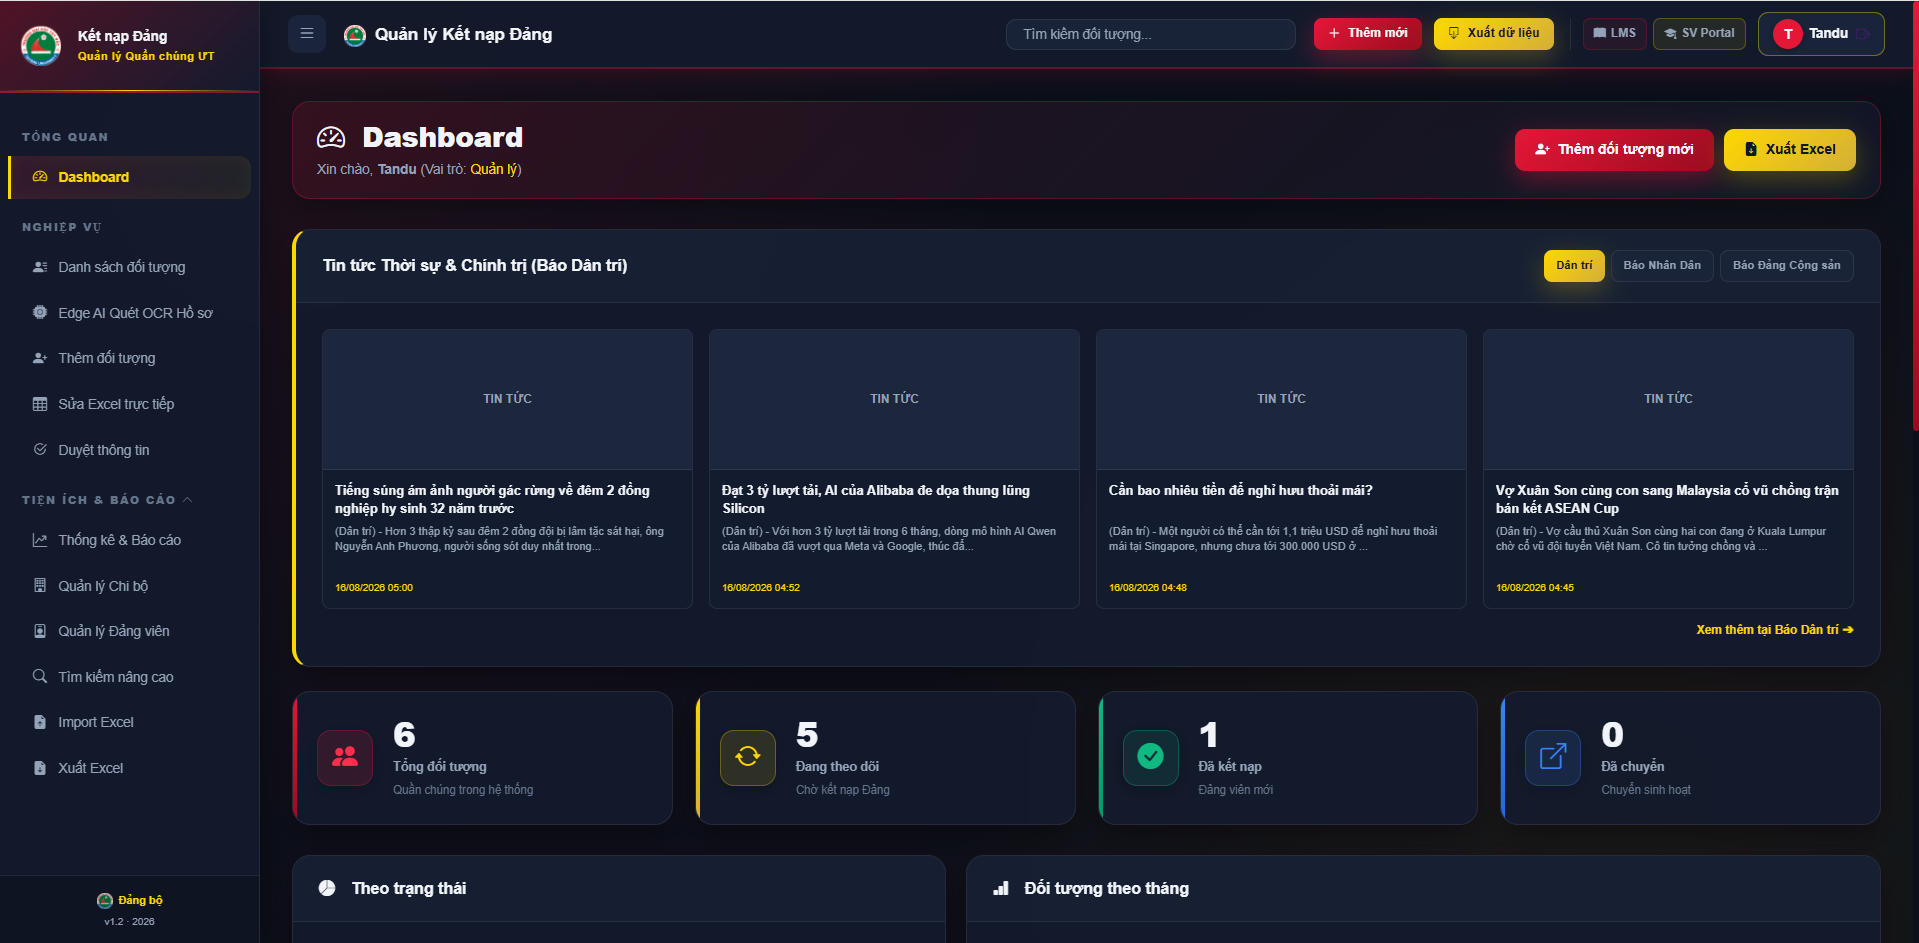
\includegraphics[width=0.98\linewidth, height=2.3cm, keepaspectratio]{giaodienquanli.png}
        \vspace{1pt}
        \fontsize{6.2pt}{7.8pt}\selectfont
        \begin{itemize}
          \setlength{\itemsep}{0.5pt}
          \item \textbf{Thống kê \& RSS}: 4 Trạng thái \& 3 Báo (*Dân trí, Nhân Dân, Báo Đảng*).
          \item \textbf{Duyệt đối chiếu 2 Tab}: \textbf{Tô màu Vàng} ô thay đổi Cũ -- Mới.
          \item \textbf{Sửa Nhanh Autosave}: Bấm sửa trực tiếp, lưu ngầm AJAX khi blur (Vàng $\to$ Xanh $\to$ Đỏ), phím tắt $\uparrow \downarrow \leftarrow \rightarrow$, xóa hàng loạt.
        \end{itemize}
      \end{greenCard}
    \end{column}
  \end{columns}
\end{frame}

% ------------------------------------------------------------------------------
% 9. EDGE AI — XỬ LÝ HÌNH ẢNH CAMERA & TIỀN XỬ LÝ CANVAS
% ------------------------------------------------------------------------------
\begin{frame}{EDGE AI — XỬ LÝ HÌNH ẢNH CAMERA \& TIỀN XỬ LÝ CANVAS}
  % Sơ đồ Pipeline xử lý ảnh
  \begin{center}
    \tikz[scale=0.88, every node/.style={transform shape, font=\fontsize{6pt}{7.5pt}\selectfont\bfseries, align=center, minimum height=0.55cm, rounded corners=2pt}]{
      \node[draw=PartyRed, fill=red!10, minimum width=2.2cm] (p1) {1. Quét Camera\\Đo nét Laplacian};
      \node[draw=GoldYellow, fill=yellow!10, minimum width=2.2cm, right=0.2cm of p1] (p2) {2. Lọc xám\\Bù sáng tự động};
      \node[draw=SkyBlue, fill=blue!10, minimum width=2.2cm, right=0.2cm of p2] (p3) {3. Nhị phân hóa\\Làm sắc nét chữ};
      \node[draw=IndigoColor, fill=IndigoColor!10, minimum width=2.2cm, right=0.2cm of p3] (p4) {4. Nắn góc nghiêng\\(Deskew)};
      \node[draw=SuccessGreen, fill=green!10, minimum width=2.2cm, right=0.2cm of p4] (p5) {5. Cắt ảnh thẻ\\Chuẩn 3x4};
      \draw[-Latex, thick, gray] (p1) -- (p2);
      \draw[-Latex, thick, gray] (p2) -- (p3);
      \draw[-Latex, thick, gray] (p3) -- (p4);
      \draw[-Latex, thick, gray] (p4) -- (p5);
    }
  \end{center}
  \vspace{-0.2cm}
  \begin{columns}[T]
    \begin{column}{0.48\textwidth}
      \begin{greenCard}{Quét Live Camera \& Đo Độ nét}
        \fontsize{6.8pt}{8.5pt}\selectfont
        \begin{itemize}
          \setlength{\itemsep}{1.2pt}
          \item Mở trực tiếp Camera qua WebRTC trên trình duyệt máy khách.
          \item \textbf{Thuật toán đo nét Laplacian ($L \ge 65\%$)}: Khung viền \textbf{\color{PartyRed}ĐỎ} khi rung mờ và tự đổi sang \textbf{\color{SuccessGreen}XANH LÁ} khi đủ nét để chụp.
          \item Tự động chặn ảnh rác không phải giấy tờ hợp lệ.
        \end{itemize}
      \end{greenCard}
    \end{column}
    \begin{column}{0.48\textwidth}
      \begin{infoCard}
        \textbf{\color{DarkRed}Đường ống Canvas \& Cắt ảnh 3x4}
        \fontsize{6.8pt}{8.5pt}\selectfont
        \begin{itemize}
          \setlength{\itemsep}{1.2pt}
          \item Lọc xám, bù sáng tự động, xóa bóng tay \& khử lóa flash.
          \item Tách nét chữ đen trên nền trắng \& làm sắc nét.
          \item \textbf{Nắn góc nghiêng (Deskew)}: Tăng $20-35\%$ độ chính xác OCR.
          \item Nhận diện khuôn mặt, cắt đúng tỷ lệ ảnh thẻ $3:4$ ($300 \times 400$px).
        \end{itemize}
      \end{infoCard}
    \end{column}
  \end{columns}
\end{frame}

% ------------------------------------------------------------------------------
% 10. EDGE AI — NHẬN DẠNG CCCD TỰ ĐIỀN FORM VÀ MINH BẠCH HÓA XAI
% ------------------------------------------------------------------------------
\begin{frame}{EDGE AI — NHẬN DẠNG CCCD TỰ ĐIỀN FORM VÀ MINH BẠCH HÓA XAI}
  \begin{columns}[T]
    \begin{column}{0.48\textwidth}
      \begin{highlightCard}{Tesseract WebAssembly (WASM) Auto-fill}
        \fontsize{6.8pt}{8.5pt}\selectfont
        \begin{itemize}
          \setlength{\itemsep}{1.5pt}
          \item \textbf{Chạy 100\% tại RAM máy khách}: Engine WASM C++ thực thi qua Web Workers, hoàn toàn không tốn tài nguyên máy chủ.
          \item \textbf{Bóc tách CCCD 2 mặt trong 2 giây}: Regex ngữ cảnh tự nhận dạng *Họ tên, Ngày sinh, Số CCCD, Giới tính, Quê quán, Lớp*.
          \item \textbf{Tự động điền 100\% Form}: Giảm 90\% công sức nhập liệu.
          \item \textbf{Bảo vệ quyền riêng tư}: Không gửi ảnh CCCD thô lên server.
        \end{itemize}
      \end{highlightCard}
    \end{column}
    \begin{column}{0.48\textwidth}
      \begin{greenCard}{Minh bạch hóa AI (Explainable AI - XAI)}
        \begin{center}
          \tikz[scale=0.82, every node/.style={transform shape, font=\tiny\bfseries, align=center}]{
            \node[draw=SuccessGreen, fill=green!10, rounded corners=2pt, minimum width=1.4cm] (c1) {Xanh lá\\$\ge 85\%$ (An toàn)};
            \node[draw=GoldYellow, fill=yellow!10, rounded corners=2pt, minimum width=1.4cm, right=0.15cm of c1] (c2) {Vàng\\$60-84\%$ (Xem lại)};
            \node[draw=PartyRed, fill=red!10, rounded corners=2pt, minimum width=1.4cm, right=0.15cm of c2] (c3) {Đỏ\\$<60\%$ (Bắt lỗi)};
          }
        \end{center}
        \fontsize{6.5pt}{8pt}\selectfont
        \begin{itemize}
          \setlength{\itemsep}{1pt}
          \item \textbf{Xóa bỏ "hộp đen"}: Phủ Bounding Box 3 màu quanh từng từ.
          \item Rê chuột lên từng từ xem chữ gốc và điểm tin cậy thực tế.
          \item Ghi nhận vết nhật ký vào bảng `edge\_ai\_logs`.
        \end{itemize}
      \end{greenCard}
    \end{column}
  \end{columns}
\end{frame}

% ------------------------------------------------------------------------------
% 11. AGENT AI — HỆ THỐNG THẨM ĐỊNH HỒ SƠ MINH CHỨNG ĐA TÁC TỬ
% ------------------------------------------------------------------------------
\begin{frame}{AGENT AI — HỆ THỐNG THẨM ĐỊNH HỒ SƠ MINH CHỨNG ĐA TÁC TỬ}
  % Sơ đồ Multi-Agent
  \begin{center}
    \tikz[scale=0.88, every node/.style={transform shape, font=\fontsize{6pt}{7.5pt}\selectfont\bfseries, align=center, minimum height=0.55cm, rounded corners=2pt}]{
      \node[draw=NavyBlue, fill=blue!10, minimum width=2.4cm] (a1) {1. Synopsis Agent\\(Nhận diện mẫu)};
      \node[draw=SkyBlue, fill=cyan!10, minimum width=2.4cm, right=0.2cm of a1] (a2) {2. Field Extractor\\(Trích xuất dữ liệu)};
      \node[draw=GoldYellow, fill=yellow!10, minimum width=2.4cm, right=0.2cm of a2] (a3) {3. Gap Diagnostic\\(Bắt lỗi ô khuyết)};
      \node[draw=PartyRed, fill=red!10, minimum width=2.4cm, right=0.2cm of a3] (a4) {4. Executive Synthesis\\(Phán quyết kết luận)};
      \draw[-Latex, thick, gray] (a1) -- (a2);
      \draw[-Latex, thick, gray] (a2) -- (a3);
      \draw[-Latex, thick, gray] (a3) -- (a4);
    }
  \end{center}
  \vspace{-0.2cm}
  \begin{columns}[T]
    \begin{column}{0.50\textwidth}
      \begin{infoCard}
        \textbf{\color{DarkRed}Vai trò 4 Tác tử AI Phối hợp}
        \fontsize{6.8pt}{8.5pt}\selectfont
        \begin{enumerate}
          \setlength{\itemsep}{1pt}
          \item \textbf{Synopsis}: Quét nhận diện mẫu trong 10 mẫu hồ sơ.
          \item \textbf{Field Extractor}: Bóc tách Họ tên, Ngày sinh, Điểm...
          \item \textbf{Gap Diagnostic}: Bắt lỗi chấm lửng (\texttt{.....}), ô trống.
          \item \textbf{Executive Synthesis}: Đánh giá \% hoàn thiện.
        \end{enumerate}
      \end{infoCard}
    \end{column}
    \begin{column}{0.48\textwidth}
      \begin{highlightCard}{Phán quyết Đồng thuận \& Xuất kết quả}
        \fontsize{6.8pt}{8.5pt}\selectfont
        \begin{itemize}
          \setlength{\itemsep}{1.2pt}
          \item \textbf{\color{SuccessGreen}HỒ SƠ ĐẠT}: Đủ 100\% thông tin, đủ dấu \& chữ ký.
          \item \textbf{\color{GoldYellow}CẦN BỔ SUNG}: Thiếu mục phụ (hướng dẫn cụ thể).
          \item \textbf{\color{PartyRed}KHÔNG HỢP LỆ}: Thiếu thông tin cốt lõi hoặc thiếu dấu.
        \end{itemize}
        \textit{Xuất kết quả JSON, CSV, sao chép Clipboard \& ghi log CSDL.}
      \end{highlightCard}
    \end{column}
  \end{columns}
\end{frame}

% ------------------------------------------------------------------------------
% 12. AGENT AI — TÁC TỬ TỰ ĐỘNG ÁNH XẠ TIÊU ĐỀ CỘT EXCEL
% ------------------------------------------------------------------------------
\begin{frame}{AGENT AI — TÁC TỬ TỰ ĐỘNG ÁNH XẠ TIÊU ĐỀ CỘT EXCEL}
  \begin{columns}[T]
    \begin{column}{0.48\textwidth}
      \begin{highlightCard}{Tác tử Ánh xạ Cột AI (\texttt{excel\_column\_agent.js})}
        \fontsize{6.8pt}{8.5pt}\selectfont
        \begin{itemize}
          \setlength{\itemsep}{1.5pt}
          \item \textbf{Nhập liệu hàng loạt}: Nạp danh sách hàng trăm sinh viên từ file Excel/CSV bằng 1 thao tác kéo thả.
          \item \textbf{Tự nhận diện tiêu đề biến thể}:
                \begin{itemize}
                  \item Chuẩn hóa Unicode, loại bỏ ký tự lạ.
                  \item Đối soát với từ điển 35 trường CSDL MySQL để nhận diện tên viết tắt (\texttt{MSSV}, \texttt{Hoten}, \texttt{Qli}...).
                \end{itemize}
          \item \textbf{Cảnh báo cột khuyết}: Gắn nhãn viền đỏ \texttt{[Cột A - Chưa có tiêu đề]}.
        \end{itemize}
      \end{highlightCard}
    \end{column}
    \begin{column}{0.48\textwidth}
      \begin{greenCard}{Giao diện Modal Đối chiếu 2 Cột Trực quan}
        \begin{center}
          \tikz[scale=0.82, every node/.style={transform shape, font=\tiny\bfseries, align=center}]{
            \node[draw=NavyBlue, fill=blue!5, rounded corners=2pt, minimum width=2.0cm] (e) {Cột file Excel\\(\texttt{MSSV}, \texttt{Hoten})};
            \node[draw=GoldYellow, fill=yellow!15, rounded corners=2pt, minimum width=1.5cm, right=0.3cm of e] (m) {AI Matching\\(Tự động khớp)};
            \node[draw=SuccessGreen, fill=green!5, rounded corners=2pt, minimum width=2.0cm, right=0.3cm of m] (d) {Trường MySQL\\(\texttt{ma\_sv}, \texttt{ho\_ten})};
            \draw[-Latex, thick, gray] (e) -- (m);
            \draw[-Latex, thick, gray] (m) -- (d);
          }
        \end{center}
        \fontsize{6.5pt}{8pt}\selectfont
        \begin{itemize}
          \setlength{\itemsep}{1pt}
          \item Cho phép quản lý đổi lại trường CSDL trước khi lưu.
          \item Xem trước 10 dòng đầu \& Chặn trùng lặp Mã SV.
        \end{itemize}
      \end{greenCard}
    \end{column}
  \end{columns}
\end{frame}

% ------------------------------------------------------------------------------
% 13. PYTHON MICROSERVICE — KIẾN TRÚC DỊCH VỤ VÀ PHP PROXY BRIDGE
% ------------------------------------------------------------------------------
\begin{frame}{PYTHON MICROSERVICE — KIẾN TRÚC DỊCH VỤ VÀ PHP PROXY BRIDGE}
  \begin{columns}[T]
    \begin{column}{0.48\textwidth}
      \begin{infoCard}
        \textbf{\color{DarkRed}Kiến trúc Microservice-Lite Độc lập}
        \fontsize{6.8pt}{8.5pt}\selectfont
        \begin{itemize}
          \setlength{\itemsep}{2pt}
          \item \textbf{Máy chủ Python Flask :5000}: Chạy nền chuyên trách toàn bộ tác vụ xử lý tệp nặng (tạo PDF và bảng tính Excel lớn).
          \item \textbf{Tách biệt tải nặng}: Giải phóng máy chủ Web PHP khỏi các phép tính render vector tốn CPU, Web luôn phản hồi $<0.3$s.
          \item \textbf{Cô lập lỗi hoàn toàn}: Nếu render file gặp sự cố, hệ thống Web chính vẫn vận hành an toàn 100\%.
        \end{itemize}
      \end{infoCard}
    \end{column}
    \begin{column}{0.48\textwidth}
      \begin{greenCard}{Cơ chế Cầu nối Proxy (\texttt{api\_proxy.php})}
        \begin{center}
          \tikz[scale=0.82, every node/.style={transform shape, font=\tiny\bfseries, align=center}]{
            \node[draw=NavyBlue, fill=blue!5, rounded corners=2pt, minimum width=1.5cm] (c) {Client\\Browser};
            \node[draw=DarkRed, fill=red!5, rounded corners=2pt, minimum width=1.8cm, right=0.35cm of c] (p) {PHP Backend\\(\texttt{api\_proxy})};
            \node[draw=SuccessGreen, fill=green!5, rounded corners=2pt, minimum width=1.8cm, right=0.35cm of p] (py) {Python Flask\\(:5000 Engine)};
            \draw[-Latex, thick, NavyBlue] (c) -- (p);
            \draw[-Latex, thick, DarkRed] (p) -- (py);
            \path (c.north east) -- node[above=1.5pt, font=\fontsize{4.5pt}{5.5pt}\selectfont, color=NavyBlue]{Request} (p.north west);
            \path (p.north east) -- node[above=1.5pt, font=\fontsize{4.5pt}{5.5pt}\selectfont, color=DarkRed]{REST JSON} (py.north west);
            \draw[-Latex, thick, SuccessGreen, dashed] (py.south) to[bend left=30] node[below=1.5pt, font=\fontsize{4.5pt}{5.5pt}\selectfont, color=SuccessGreen]{Binary Stream} (c.south);
          }
        \end{center}
        \fontsize{6.5pt}{8pt}\selectfont
        \textbf{Nguyên lý}: PHP đóng gói dữ liệu CSDL gửi JSON $\to$ Python render file nhị phân $\to$ Trả về Client tải xuống tức thì.
      \end{greenCard}
    \end{column}
  \end{columns}
\end{frame}

% ------------------------------------------------------------------------------
% 14. PYTHON MICROSERVICE — XỬ LÝ LOGIC BACKEND VÀ KẾT XUẤT TÀI LIỆU
% ------------------------------------------------------------------------------
\begin{frame}{PYTHON MICROSERVICE — XỬ LÝ LOGIC BACKEND VÀ KẾT XUẤT TÀI LIỆU}
  \begin{columns}[T]
    \begin{column}{0.48\textwidth}
      \begin{highlightCard}{Xử lý Nghiệp vụ Backend \& Excel (\texttt{openpyxl})}
        \fontsize{6.6pt}{8.1pt}\selectfont
        \begin{itemize}
          \setlength{\itemsep}{1.2pt}
          \item \textbf{Logic thẩm định dữ liệu đa bảng}: Tự động gom nhóm thông tin cá nhân, điểm rèn luyện, kết quả học lớp Đảng và kiểm tra mốc thời gian hợp lệ trước khi kết xuất.
          \item \textbf{Báo cáo Excel 35 Cột}:
                \begin{itemize}
                  \item Xuất trọn vẹn 35 cột thuộc tính CSDL MySQL trong \textbf{0.32 giây}.
                  \item Header đỏ cờ trang nghiêm, thuật toán Auto-fit tự co giãn độ rộng cột theo ký tự thực tế.
                  \item 3 Chế độ xuất: Toàn trường, theo Chi bộ, theo Lớp.
                \end{itemize}
        \end{itemize}
      \end{highlightCard}
    \end{column}
    \begin{column}{0.50\textwidth}
      \begin{greenCard}{Kết xuất 8 Mẫu phiếu PDF (\texttt{ReportLab})}
        \fontsize{6.4pt}{7.8pt}\selectfont
        \begin{itemize}
          \setlength{\itemsep}{0.8pt}
          \item \textbf{ReportLab Vector Canvas}: Định vị tọa độ mm trên khổ A4 chuẩn thể thức văn bản hành chính Đảng.
          \item \textbf{Đóng khung đỏ nổi bật}: Tự động điền dữ liệu CSDL và \textbf{\color{PartyRed}bôi đỏ [ Dữ liệu ]} giúp nhận diện dễ dàng để sao chép.
          \item \textbf{Trọn bộ 8 biểu mẫu}: Đơn (1-KNĐ), Lý lịch 3 đời (2-KNĐ), Giới thiệu (3-KNĐ), Nghị quyết Đoàn TN (4-KNĐ), Công đoàn (4a-KNĐ), Nhận xét Chi ủy (5-KNĐ), Chứng nhận học lớp Đảng (CN-NTVĐ1 \& 2).
        \end{itemize}
      \end{greenCard}
    \end{column}
  \end{columns}
\end{frame}

% ------------------------------------------------------------------------------
% 15. ĐÁNH GIÁ HIỆU NĂNG, TÍNH KHẢ THI VÀ GIÁ TRỊ THỰC TIỄN ĐỘT PHÁ
% ------------------------------------------------------------------------------
\begin{frame}{ĐÁNH GIÁ HIỆU NĂNG, TÍNH KHẢ THI VÀ GIÁ TRỊ THỰC TIỄN ĐỘT PHÁ}
  \begin{columns}[T]
    \begin{column}{0.54\textwidth}
      \begin{greenCard}{Bảng Đối sánh Benchmark Định lượng}
        \fontsize{6.2pt}{7.6pt}\selectfont
        \begin{tabularx}{\linewidth}{Xcc}
          \toprule
          \textbf{Chỉ số Đánh giá} & \textbf{Thủ công} & \textbf{QLUT-Đảng}        \\
          \midrule
          1. Nhập liệu CCCD / SV   & 45--60 phút       & \textbf{$<2.5$ giây}      \\
          2. Rà soát lỗi hồ sơ     & 30--45 phút       & \textbf{$<5.0$ giây}      \\
          3. Xuất 8 PDF \& Excel   & Vài giờ           & \textbf{0.32--1.0 giây}   \\
          4. Chi phí Server AI GPU & Rất đắt           & \textbf{0 VNĐ (WASM)}     \\
          5. Độ chính xác bóc tách & Sai sót mắt       & \textbf{$\ge 95\%$ (XAI)} \\
          6. Toàn vẹn CSDL         & Phân tán          & \textbf{100\% (3NF)}      \\
          \bottomrule
        \end{tabularx}
      \end{greenCard}
    \end{column}
    \begin{column}{0.44\textwidth}
      \begin{highlightCard}{Giá trị Thực tiễn Đột phá}
        \fontsize{6.6pt}{8.2pt}\selectfont
        \begin{itemize}
          \setlength{\itemsep}{1.2pt}
          \item \textbf{Tiết kiệm 95\% thời gian}: Giải phóng hàng trăm giờ hành chính cho Bí thư và Đảng ủy.
          \item \textbf{Minh bạch \& Chuẩn hóa}: Xóa bỏ hoàn toàn nguy cơ thất lạc hồ sơ giấy tờ nhiều năm.
          \item \textbf{Khả năng nhân rộng}: Sẵn sàng triển khai mở rộng cho toàn bộ các Chi bộ trong Nhà trường.
        \end{itemize}
      \end{highlightCard}
    \end{column}
  \end{columns}
\end{frame}

% ------------------------------------------------------------------------------
% SLIDE KẾT THÚC (THANK YOU SLIDE)
% ------------------------------------------------------------------------------
\begin{frame}[plain]
  \vspace{0.6cm}
  \centering
  {\fontsize{18pt}{22pt}\selectfont\bfseries\color{DarkRed} XIN TRÂN TRỌNG CẢM ƠN!}\\
  \vspace{0.25cm}
  {\fontsize{10.5pt}{12.5pt}\selectfont\color{TextDark} Kính chúc Quý Thầy Cô và Hội đồng sức khỏe và công tác tốt!}

  \vspace{0.4cm}
  \tikz \draw[PartyRed, line width=1.5pt] (0,0) -- (8cm, 0);
  \vspace{0.4cm}

  \begin{infoCard}[width=10.5cm]
    \centering
    \fontsize{9.5pt}{11.5pt}\selectfont\bfseries\color{DarkRed}
    NHÓM 02 SẴN SÀNG LẮNG NGHE Ý KIẾN ĐÓNG GÓP VÀ GIẢI ĐÁP CÂU HỎI (Q\&A)
  \end{infoCard}

  \vspace{0.3cm}
  {\fontsize{8pt}{10pt}\selectfont\color{gray} Khoa Công nghệ Thông tin --- Trường Đại học Tây Bắc}
\end{frame}

\end{document}
